%----------------------------------------------------------------------------------------
% Parallel Gaussian Elim using OpenMP
%----------------------------------------------------------------------------------------

\section{Parallel Gaussian elimination using OpenMP}

\subsection{Add OpenMP directives to parallelize the \emph{Guassian\_elim} function}

\vspace{0.5cm}
\lstinputlisting[
	style=CStyle,
	firstline=117, % First line of code
	lastline=138, % Lastl ine of code
	caption=Parallelizing Gaussian\_elim (line 117-138 in lab3part5.c), % Caption above the listing
	label=lst:lab3part5a, % Label for referencing this listing
	frame=single, % Frame around the code listing
	showstringspaces=false, % Don't put marks in string spaces
	numbers=left, % Line numbers on left
	numberstyle=\normalsize % Line numbers styling
	]{../code/lab3part5.c}

\subsection{Add OpenMP directives to parallelize the \emph{Row\_solve} function}

\vspace{0.5cm}
\lstinputlisting[
	style=CStyle,
	firstline=140, % First line of code
	lastline=165, % Lastl ine of code
	caption=Parallelizing Row\_solve (line 140-165 in lab3part5.c), % Caption above the listing
	label=lst:lab3part5a, % Label for referencing this listing
	frame=single, % Frame around the code listing
	showstringspaces=false, % Don't put marks in string spaces
	numbers=left, % Line numbers on left
	numberstyle=\normalsize % Line numbers styling
	]{../code/lab3part5.c}

\subsection{Compile and run your code. Use a matrix size $10^3 \times 10^3$.
Tabulate the performance and speedup for 1,2,4,8 threads}

\begin{figure*}[ht]
	\centering
	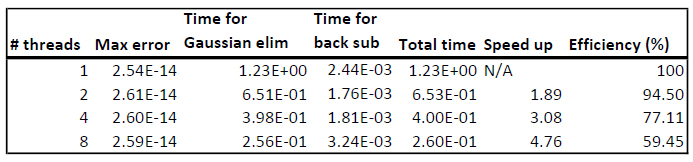
\includegraphics[width=\textwidth]{graphics/P5_c_table.PNG}
	\label{fig:lab3part3c_i}
\end{figure*}

\begin{figure}[ht]
	\centering
	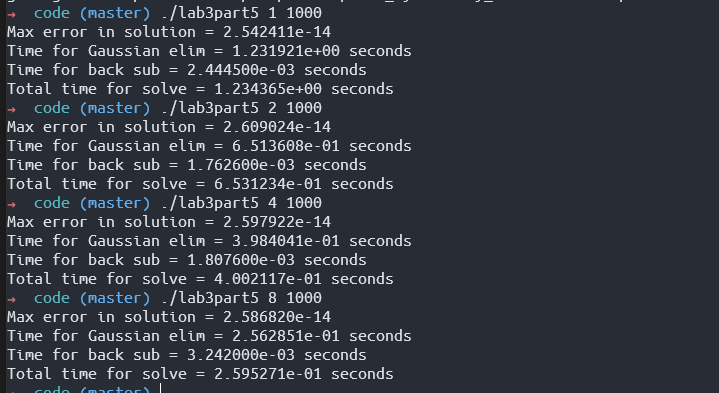
\includegraphics[width=\textwidth]{graphics/P5_c_terminal_output.PNG}
	\caption{Terminal output for execution with 1, 2, 4, 8 threads respectively,
	for a matrix size $10^3 \times 10^3$}
	\label{fig:lab3part3c_ii}
\end{figure}

\begin{figure}[ht]
	\centering
	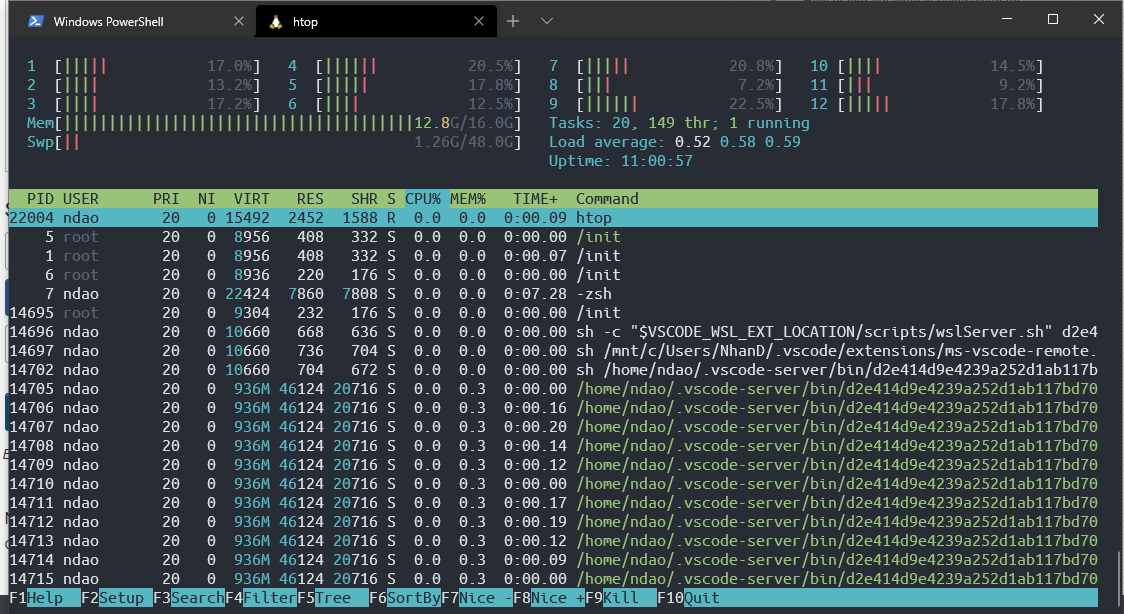
\includegraphics[width=\textwidth]{graphics/P5_c_cores.PNG}
	\caption{Number of cores using htop}
	\label{fig:lab3part3c_iii}
\end{figure}

\subsubsection{At what point does the speedup stop increasing?}
Speedup stop increasing at after 10 threads.

\subsubsection{Is this consistent with the number of cores?}
As seen in \cref{fig:lab3part3c_iii} there are 12 available cores,
hence it is consistent with the number of cores as the speedup seems
to stop increasing after 10 threads which is close to the number
of available cores.


